\documentclass[]{article}
\usepackage{lmodern}
\usepackage{amssymb,amsmath}
\usepackage{ifxetex,ifluatex}
\usepackage{fixltx2e} % provides \textsubscript
\ifnum 0\ifxetex 1\fi\ifluatex 1\fi=0 % if pdftex
  \usepackage[T1]{fontenc}
  \usepackage[utf8]{inputenc}
\else % if luatex or xelatex
  \ifxetex
    \usepackage{mathspec}
  \else
    \usepackage{fontspec}
  \fi
  \defaultfontfeatures{Ligatures=TeX,Scale=MatchLowercase}
\fi
% use upquote if available, for straight quotes in verbatim environments
\IfFileExists{upquote.sty}{\usepackage{upquote}}{}
% use microtype if available
\IfFileExists{microtype.sty}{%
\usepackage{microtype}
\UseMicrotypeSet[protrusion]{basicmath} % disable protrusion for tt fonts
}{}
\usepackage[margin=0.6in]{geometry}
\usepackage{hyperref}
\hypersetup{unicode=true,
            pdftitle={Large-Sample Normal Approximation to the Posterior},
            pdfborder={0 0 0},
            breaklinks=true}
\urlstyle{same}  % don't use monospace font for urls
\usepackage{color}
\usepackage{fancyvrb}
\newcommand{\VerbBar}{|}
\newcommand{\VERB}{\Verb[commandchars=\\\{\}]}
\DefineVerbatimEnvironment{Highlighting}{Verbatim}{commandchars=\\\{\}}
% Add ',fontsize=\small' for more characters per line
\usepackage{framed}
\definecolor{shadecolor}{RGB}{248,248,248}
\newenvironment{Shaded}{\begin{snugshade}}{\end{snugshade}}
\newcommand{\KeywordTok}[1]{\textcolor[rgb]{0.13,0.29,0.53}{\textbf{#1}}}
\newcommand{\DataTypeTok}[1]{\textcolor[rgb]{0.13,0.29,0.53}{#1}}
\newcommand{\DecValTok}[1]{\textcolor[rgb]{0.00,0.00,0.81}{#1}}
\newcommand{\BaseNTok}[1]{\textcolor[rgb]{0.00,0.00,0.81}{#1}}
\newcommand{\FloatTok}[1]{\textcolor[rgb]{0.00,0.00,0.81}{#1}}
\newcommand{\ConstantTok}[1]{\textcolor[rgb]{0.00,0.00,0.00}{#1}}
\newcommand{\CharTok}[1]{\textcolor[rgb]{0.31,0.60,0.02}{#1}}
\newcommand{\SpecialCharTok}[1]{\textcolor[rgb]{0.00,0.00,0.00}{#1}}
\newcommand{\StringTok}[1]{\textcolor[rgb]{0.31,0.60,0.02}{#1}}
\newcommand{\VerbatimStringTok}[1]{\textcolor[rgb]{0.31,0.60,0.02}{#1}}
\newcommand{\SpecialStringTok}[1]{\textcolor[rgb]{0.31,0.60,0.02}{#1}}
\newcommand{\ImportTok}[1]{#1}
\newcommand{\CommentTok}[1]{\textcolor[rgb]{0.56,0.35,0.01}{\textit{#1}}}
\newcommand{\DocumentationTok}[1]{\textcolor[rgb]{0.56,0.35,0.01}{\textbf{\textit{#1}}}}
\newcommand{\AnnotationTok}[1]{\textcolor[rgb]{0.56,0.35,0.01}{\textbf{\textit{#1}}}}
\newcommand{\CommentVarTok}[1]{\textcolor[rgb]{0.56,0.35,0.01}{\textbf{\textit{#1}}}}
\newcommand{\OtherTok}[1]{\textcolor[rgb]{0.56,0.35,0.01}{#1}}
\newcommand{\FunctionTok}[1]{\textcolor[rgb]{0.00,0.00,0.00}{#1}}
\newcommand{\VariableTok}[1]{\textcolor[rgb]{0.00,0.00,0.00}{#1}}
\newcommand{\ControlFlowTok}[1]{\textcolor[rgb]{0.13,0.29,0.53}{\textbf{#1}}}
\newcommand{\OperatorTok}[1]{\textcolor[rgb]{0.81,0.36,0.00}{\textbf{#1}}}
\newcommand{\BuiltInTok}[1]{#1}
\newcommand{\ExtensionTok}[1]{#1}
\newcommand{\PreprocessorTok}[1]{\textcolor[rgb]{0.56,0.35,0.01}{\textit{#1}}}
\newcommand{\AttributeTok}[1]{\textcolor[rgb]{0.77,0.63,0.00}{#1}}
\newcommand{\RegionMarkerTok}[1]{#1}
\newcommand{\InformationTok}[1]{\textcolor[rgb]{0.56,0.35,0.01}{\textbf{\textit{#1}}}}
\newcommand{\WarningTok}[1]{\textcolor[rgb]{0.56,0.35,0.01}{\textbf{\textit{#1}}}}
\newcommand{\AlertTok}[1]{\textcolor[rgb]{0.94,0.16,0.16}{#1}}
\newcommand{\ErrorTok}[1]{\textcolor[rgb]{0.64,0.00,0.00}{\textbf{#1}}}
\newcommand{\NormalTok}[1]{#1}
\usepackage{graphicx,grffile}
\makeatletter
\def\maxwidth{\ifdim\Gin@nat@width>\linewidth\linewidth\else\Gin@nat@width\fi}
\def\maxheight{\ifdim\Gin@nat@height>\textheight\textheight\else\Gin@nat@height\fi}
\makeatother
% Scale images if necessary, so that they will not overflow the page
% margins by default, and it is still possible to overwrite the defaults
% using explicit options in \includegraphics[width, height, ...]{}
\setkeys{Gin}{width=\maxwidth,height=\maxheight,keepaspectratio}
\IfFileExists{parskip.sty}{%
\usepackage{parskip}
}{% else
\setlength{\parindent}{0pt}
\setlength{\parskip}{6pt plus 2pt minus 1pt}
}
\setlength{\emergencystretch}{3em}  % prevent overfull lines
\providecommand{\tightlist}{%
  \setlength{\itemsep}{0pt}\setlength{\parskip}{0pt}}
\setcounter{secnumdepth}{0}
% Redefines (sub)paragraphs to behave more like sections
\ifx\paragraph\undefined\else
\let\oldparagraph\paragraph
\renewcommand{\paragraph}[1]{\oldparagraph{#1}\mbox{}}
\fi
\ifx\subparagraph\undefined\else
\let\oldsubparagraph\subparagraph
\renewcommand{\subparagraph}[1]{\oldsubparagraph{#1}\mbox{}}
\fi

%%% Use protect on footnotes to avoid problems with footnotes in titles
\let\rmarkdownfootnote\footnote%
\def\footnote{\protect\rmarkdownfootnote}

%%% Change title format to be more compact
\usepackage{titling}

% Create subtitle command for use in maketitle
\newcommand{\subtitle}[1]{
  \posttitle{
    \begin{center}\large#1\end{center}
    }
}

\setlength{\droptitle}{-2em}

  \title{Large-Sample Normal Approximation to the Posterior}
    \pretitle{\vspace{\droptitle}\centering\huge}
  \posttitle{\par}
    \author{}
    \preauthor{}\postauthor{}
    \date{}
    \predate{}\postdate{}
  
\usepackage{multicol}

\begin{document}
\maketitle

\def\simiid{\stackrel{{\mbox{\text{\tiny i.i.d.}}}}{\sim}}

\subsection{Basic Result (rough
statement)}\label{basic-result-rough-statement}

For large sample size, the posterior distribution is approximately
\(\Theta | X_1, \ldots, X_n \sim \text{Normal}(\hat{\theta}^{MLE}, \cdots)\)

\paragraph{Binomial Model: M\&M's (Lab
7b)}\label{binomial-model-mms-lab-7b}

\begin{itemize}
\tightlist
\item
  As a class, we had x = 138 blue M\&Ms in a sample of size n = 541.
\item
  Data Model: \(X | \Theta = \theta \sim \text{Binomial}(541, \theta)\)
\item
  Suppose we use a noninformative prior of
  \(\Theta \sim \text{Beta}(1, 1)\)
\item
  The exact posterior is
  \(\Theta | X = 138 \sim \text{Beta}(1 + 138, 1 + 541 - 138)\)
\item
  The MLE is 138/541
\end{itemize}

\begin{Shaded}
\begin{Highlighting}[]
\KeywordTok{ggplot}\NormalTok{(}\DataTypeTok{data =} \KeywordTok{data.frame}\NormalTok{(}\DataTypeTok{theta =} \KeywordTok{c}\NormalTok{(}\DecValTok{0}\NormalTok{, }\DecValTok{1}\NormalTok{)), }\DataTypeTok{mapping =} \KeywordTok{aes}\NormalTok{(}\DataTypeTok{x =}\NormalTok{ theta)) }\OperatorTok{+}
\StringTok{  }\KeywordTok{stat_function}\NormalTok{(}\DataTypeTok{fun =}\NormalTok{ dbeta,}
    \DataTypeTok{args =} \KeywordTok{list}\NormalTok{(}\DataTypeTok{shape1 =} \DecValTok{1} \OperatorTok{+}\StringTok{ }\DecValTok{138}\NormalTok{, }\DataTypeTok{shape2 =} \DecValTok{1} \OperatorTok{+}\StringTok{ }\DecValTok{541} \OperatorTok{-}\StringTok{ }\DecValTok{138}\NormalTok{),}
    \DataTypeTok{n =} \DecValTok{1001}\NormalTok{) }\OperatorTok{+}
\StringTok{  }\KeywordTok{geom_vline}\NormalTok{(}\DataTypeTok{xintercept =} \DecValTok{138}\OperatorTok{/}\DecValTok{541}\NormalTok{, }\DataTypeTok{color =} \StringTok{"orange"}\NormalTok{, }\DataTypeTok{linetype =} \DecValTok{2}\NormalTok{) }\OperatorTok{+}
\StringTok{  }\KeywordTok{theme_bw}\NormalTok{()}
\end{Highlighting}
\end{Shaded}

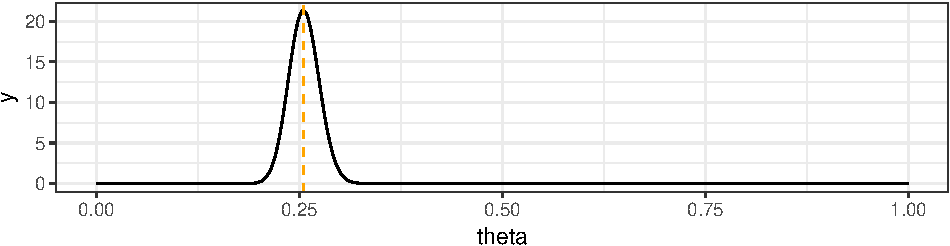
\includegraphics{20190306_normal_approx_posterior_files/figure-latex/unnamed-chunk-1-1.pdf}

\paragraph{Geometric Model: Bird Hops (Lab
8)}\label{geometric-model-bird-hops-lab-8}

\begin{itemize}
\tightlist
\item
  Observe \(X_1, \ldots, X_n\); \(X_i\) is the number of hops taken
  before bird takes off
\item
  Data Model: \(X_i | \Theta = \theta \simiid \text{Geometric}(\theta)\)
\item
  Suppose we use a noninformative prior of
  \(\Theta \sim \text{Beta}(1, 1)\)
\item
  The exact posterior is
  \(\Theta | X_1 = x_1, \ldots, X_n = x_n \sim \text{Beta}(1 + n, 1 + \sum_{i = 1}^n x_i)\)
\item
  The MLE is \(\frac{1}{1 + \bar{X}}\)
\end{itemize}

\begin{Shaded}
\begin{Highlighting}[]
\KeywordTok{ggplot}\NormalTok{(}\DataTypeTok{data =} \KeywordTok{data.frame}\NormalTok{(}\DataTypeTok{theta =} \KeywordTok{c}\NormalTok{(}\DecValTok{0}\NormalTok{, }\DecValTok{1}\NormalTok{)), }\DataTypeTok{mapping =} \KeywordTok{aes}\NormalTok{(}\DataTypeTok{x =}\NormalTok{ theta)) }\OperatorTok{+}
\StringTok{  }\KeywordTok{stat_function}\NormalTok{(}\DataTypeTok{fun =}\NormalTok{ dbeta,}
    \DataTypeTok{args =} \KeywordTok{list}\NormalTok{(}\DataTypeTok{shape1 =} \DecValTok{1} \OperatorTok{+}\StringTok{ }\KeywordTok{nrow}\NormalTok{(bird_hops), }\DataTypeTok{shape2 =} \DecValTok{1} \OperatorTok{+}\StringTok{ }\KeywordTok{sum}\NormalTok{(bird_hops}\OperatorTok{$}\NormalTok{num_hops)),}
    \DataTypeTok{n =} \DecValTok{1001}\NormalTok{) }\OperatorTok{+}
\StringTok{  }\KeywordTok{geom_vline}\NormalTok{(}\DataTypeTok{xintercept =} \DecValTok{1}\OperatorTok{/}\NormalTok{(}\DecValTok{1} \OperatorTok{+}\StringTok{ }\KeywordTok{mean}\NormalTok{(bird_hops}\OperatorTok{$}\NormalTok{num_hops)), }\DataTypeTok{color =} \StringTok{"orange"}\NormalTok{) }\OperatorTok{+}
\StringTok{  }\KeywordTok{theme_bw}\NormalTok{()}
\end{Highlighting}
\end{Shaded}

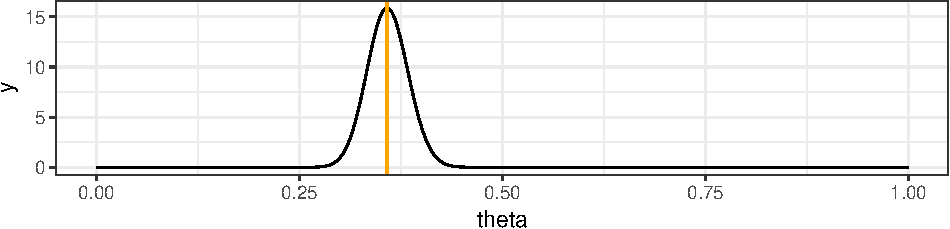
\includegraphics{20190306_normal_approx_posterior_files/figure-latex/unnamed-chunk-3-1.pdf}

\paragraph{Poisson Model: Seedlings (Lab
8)}\label{poisson-model-seedlings-lab-8}

\begin{itemize}
\tightlist
\item
  Observe \(X_1, \ldots, X_n\); \(X_i\) is the number of seedlings in
  quadrat number \(i\).
\item
  Data Model:
  \(X_i | \Lambda = \lambda \simiid \text{Poisson}(\lambda)\)
\item
  Suppose we use a noninformative prior of
  \(\Lambda \sim \text{Gamma}(1, 0.01)\)
\item
  The exact posterior is
  \(\Lambda | X_1 = x_1, \ldots, X_n = x_n \sim \text{Gamma}(1 + \sum_{i = 1}^{n} x_i, 0.01 + n)\)
\item
  The MLE is \(\bar{X}\)
\end{itemize}

\begin{Shaded}
\begin{Highlighting}[]
\KeywordTok{ggplot}\NormalTok{(}\DataTypeTok{data =} \KeywordTok{data.frame}\NormalTok{(}\DataTypeTok{theta =} \KeywordTok{c}\NormalTok{(}\DecValTok{0}\NormalTok{, }\DecValTok{2}\NormalTok{)), }\DataTypeTok{mapping =} \KeywordTok{aes}\NormalTok{(}\DataTypeTok{x =}\NormalTok{ theta)) }\OperatorTok{+}
\StringTok{  }\KeywordTok{stat_function}\NormalTok{(}\DataTypeTok{fun =}\NormalTok{ dgamma,}
    \DataTypeTok{args =} \KeywordTok{list}\NormalTok{(}\DataTypeTok{shape =} \DecValTok{1} \OperatorTok{+}\StringTok{ }\KeywordTok{sum}\NormalTok{(seedlings}\OperatorTok{$}\NormalTok{new_}\DecValTok{1993}\NormalTok{), }\DataTypeTok{rate =} \FloatTok{0.01} \OperatorTok{+}\StringTok{ }\KeywordTok{nrow}\NormalTok{(seedlings)), }\DataTypeTok{n =} \DecValTok{1001}\NormalTok{) }\OperatorTok{+}
\StringTok{  }\KeywordTok{geom_vline}\NormalTok{(}\DataTypeTok{xintercept =} \KeywordTok{mean}\NormalTok{(seedlings}\OperatorTok{$}\NormalTok{new_}\DecValTok{1993}\NormalTok{), }\DataTypeTok{color =} \StringTok{"orange"}\NormalTok{) }\OperatorTok{+}
\StringTok{  }\KeywordTok{theme_bw}\NormalTok{()}
\end{Highlighting}
\end{Shaded}

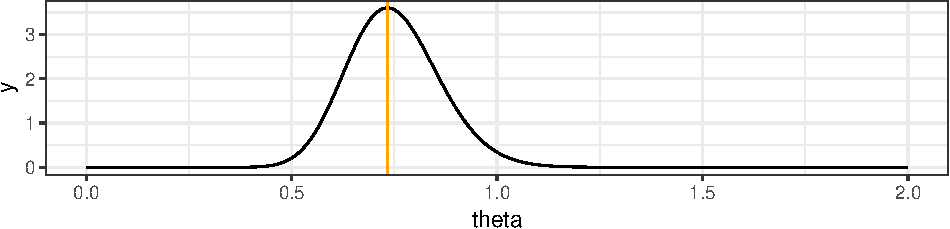
\includegraphics{20190306_normal_approx_posterior_files/figure-latex/unnamed-chunk-5-1.pdf}

\paragraph{Normal Model: Cosmic Microwave Background Radiation (Lecture,
March
4th)}\label{normal-model-cosmic-microwave-background-radiation-lecture-march-4th}

\begin{itemize}
\tightlist
\item
  Observe \(X_1, \ldots, X_n\), where \(X_i\) is the temperature
  difference in pixel \(i\).
\item
  Data Model: \(X_i \simiid \text{Normal}(\mu, \sigma^2)\)
\item
  We approximated the posterior distributions of \(\mu\) and \(\sigma\)
  by drawing samples using MCMC.
\item
  The MLEs are \(\hat{\mu}^{MLE} = \bar{X}\) and
  \(\hat{\sigma^2} = \frac{1}{n}\sum_{i=1}^n(X_i - \bar{X})^n\)
\end{itemize}

\begin{Shaded}
\begin{Highlighting}[]
\KeywordTok{ggplot}\NormalTok{() }\OperatorTok{+}
\StringTok{  }\KeywordTok{geom_density}\NormalTok{(}\DataTypeTok{data =}\NormalTok{ theta_posterior_sample, }\DataTypeTok{mapping =} \KeywordTok{aes}\NormalTok{(}\DataTypeTok{x =}\NormalTok{ mu)) }\OperatorTok{+}
\StringTok{  }\KeywordTok{geom_vline}\NormalTok{(}\DataTypeTok{xintercept =} \KeywordTok{mean}\NormalTok{(cmb}\OperatorTok{$}\NormalTok{temp_difference), }\DataTypeTok{color =} \StringTok{"orange"}\NormalTok{) }\OperatorTok{+}
\StringTok{  }\KeywordTok{theme_bw}\NormalTok{()}
\end{Highlighting}
\end{Shaded}

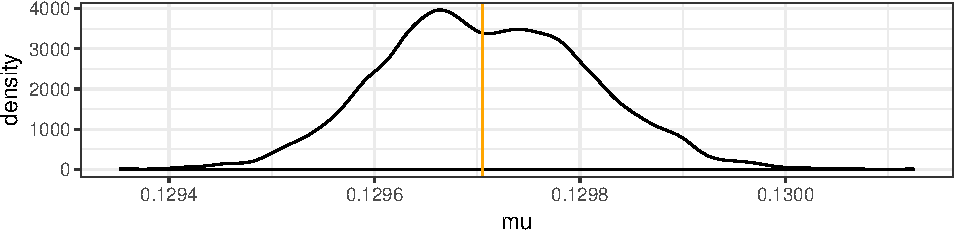
\includegraphics{20190306_normal_approx_posterior_files/figure-latex/unnamed-chunk-8-1.pdf}

\begin{Shaded}
\begin{Highlighting}[]
\KeywordTok{ggplot}\NormalTok{() }\OperatorTok{+}
\StringTok{  }\KeywordTok{geom_density}\NormalTok{(}\DataTypeTok{data =}\NormalTok{ theta_posterior_sample, }\DataTypeTok{mapping =} \KeywordTok{aes}\NormalTok{(}\DataTypeTok{x =}\NormalTok{ sigma_sq)) }\OperatorTok{+}
\StringTok{  }\KeywordTok{geom_vline}\NormalTok{(}\DataTypeTok{xintercept =} \KeywordTok{mean}\NormalTok{((cmb}\OperatorTok{$}\NormalTok{temp_difference }\OperatorTok{-}\StringTok{ }\KeywordTok{mean}\NormalTok{(cmb}\OperatorTok{$}\NormalTok{temp_difference))}\OperatorTok{^}\DecValTok{2}\NormalTok{), }\DataTypeTok{color =} \StringTok{"orange"}\NormalTok{) }\OperatorTok{+}
\StringTok{  }\KeywordTok{theme_bw}\NormalTok{()}
\end{Highlighting}
\end{Shaded}

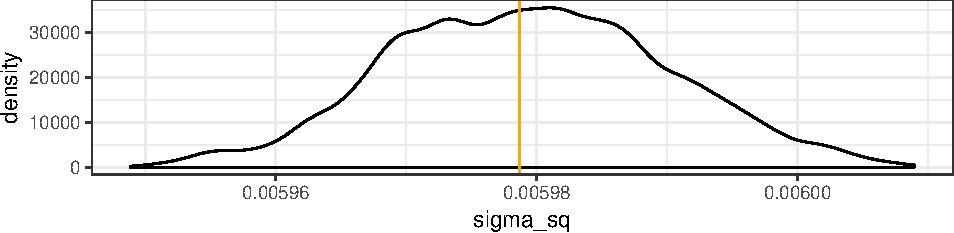
\includegraphics{20190306_normal_approx_posterior_files/figure-latex/unnamed-chunk-9-1.pdf}


\end{document}
